% !TEX root = ../thesis.tex
\chapter{Web application - BotBuster}
\label{capitolo7}
\thispagestyle{empty}
This chapter represents the practical application of our work. We wanted to provide a tangible proof the thesis, an instrument available to every users in search of classification, among the accounts met on Twitter.
We thought it was useful to allow people to be aware about the nature of the users that populate the social network.
Bots often don't claim themselves as automated accounts, that makes hard their detection, even for an experienced utilizer.


\textbf{BotBuster} is the name of the project, whose goal is to provide the probability-based classification of the desired Twitter user.
The logo used to represent the application tool is shown in Figure \ref{fig:botbuster}
The probabilities are shown in a histogram-shaped graph, with different colours, one for each target, as displayed in Figure\ref{fig:histogram}.

\begin{figure}
	\begin{center}
		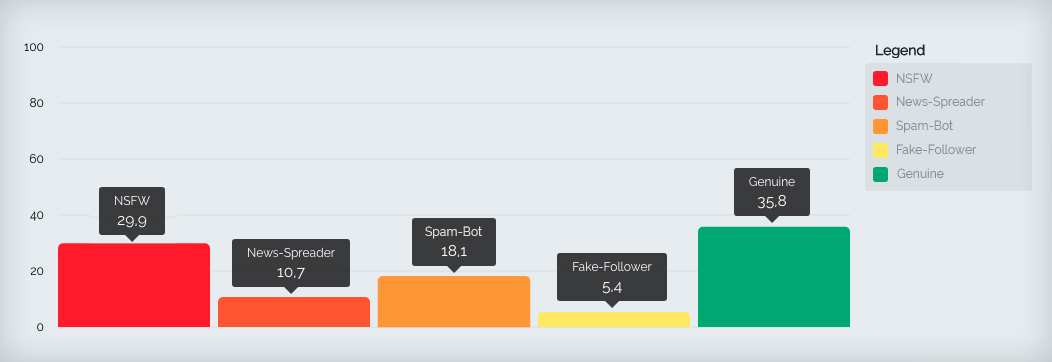
\includegraphics[width=\columnwidth]{chapter7/figure/histogram.jpg}\par 
	\end{center}
	\caption{Probability classification diagram on BotBuster}
	\label{fig:histogram}
\end{figure}

\begin{figure}
	\begin{center}
		
\includegraphics[width=\columnwidth]{chapter7/figure/logo.png}\par 
	\end{center}
	\caption{BotBuster logo}
	\label{fig:botbuster}
\end{figure}

The web application had to be visible on a public URL. It is currently available on \href{http://www.botbuster.it}{\textit{www.botbuster.it}}.

Basically, the functioning of BotBuster can be resumed in getting a Twitter user name through an input filed on the home page, and then executing the prediction pipeline described in chapter \ref{predicion_pipeline}.
The input filed filling triggers the engine operating in the background, which runs a Python script performing the prediction.
\section{Architecture}
The web application works under a client - server paradigm. The Angular program is executed on the client's web browser, while on the server runs the Flask application.
Every time a user search for a Twitter user name, the HTTP protocols is involved to perform POST and GET requests between client and server. The frontend and the backend applications handle the request and exchange, as shown in Figure\ref{fig:architecture}.
\begin{figure}[t!]
	\begin{center}
		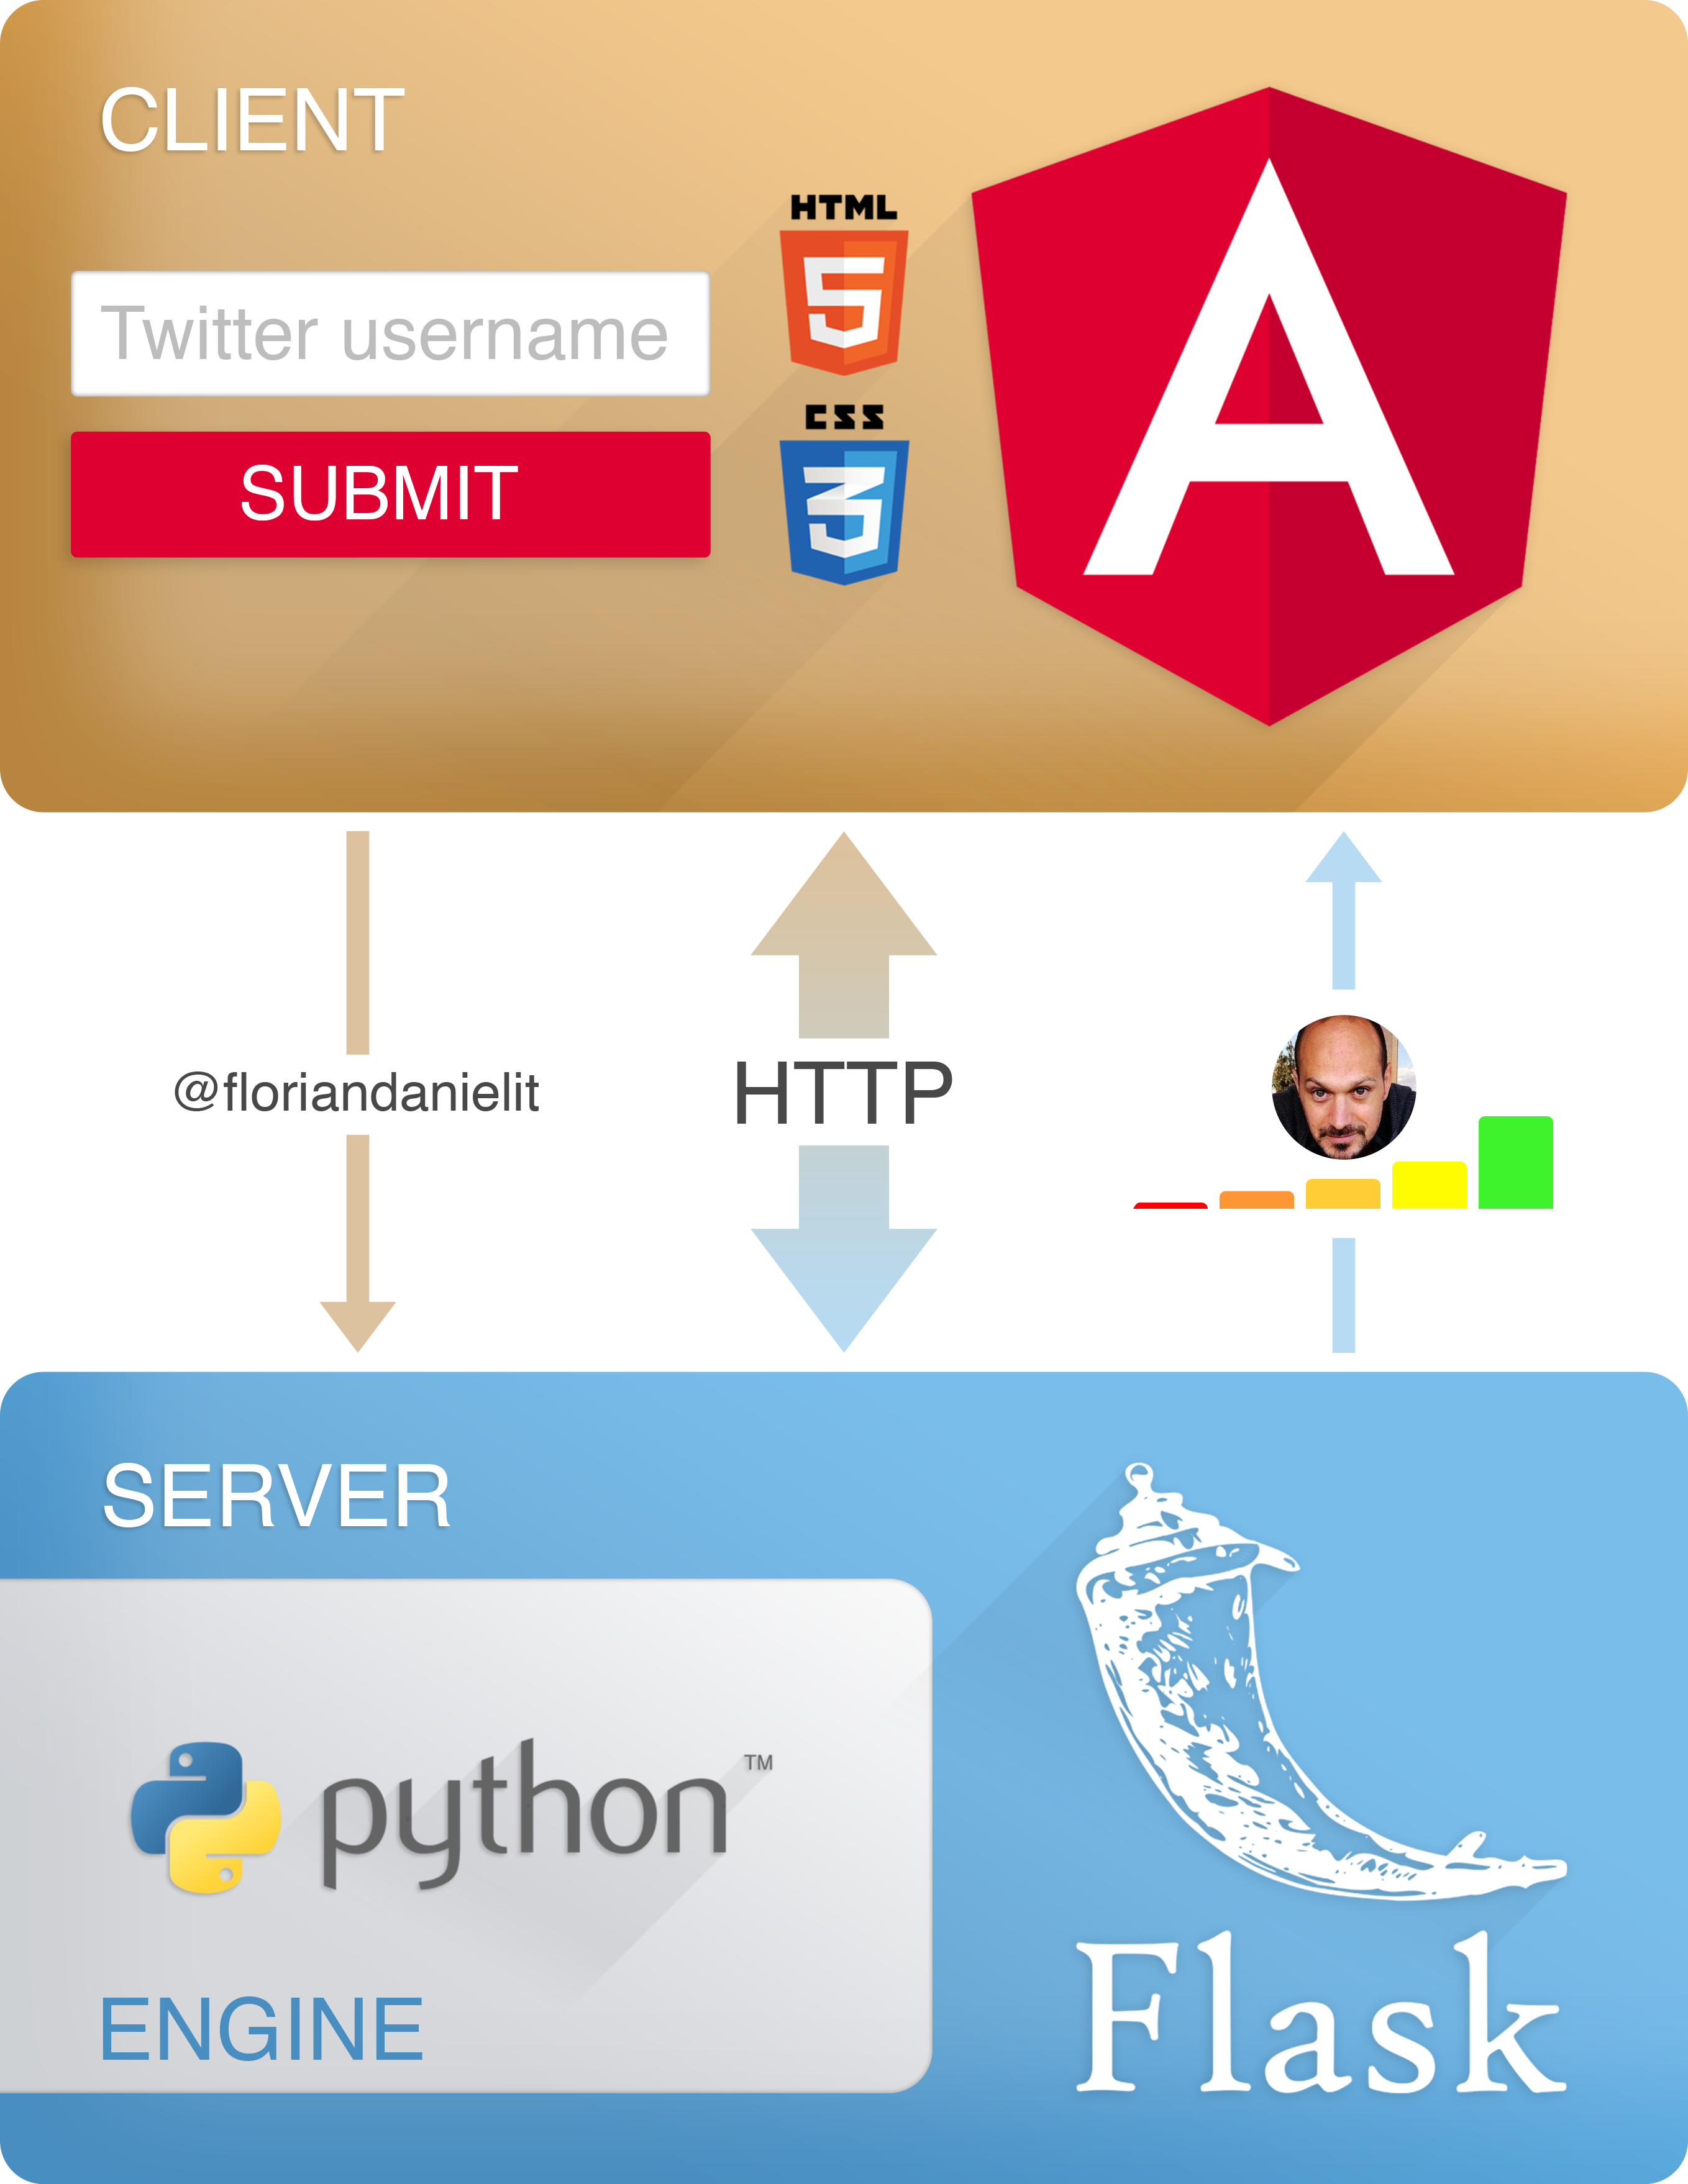
\includegraphics[width=0.6\columnwidth]{chapter7/figure/architecture.png} 
	\end{center}
	\caption{Client - Server architecture}
	\label{fig:architecture}
\end{figure}

\section{Backend}
The back-end side of the web application is the core of the whole tool. Its goal is to summarize and perform the methods explained in the previous chapters and to classify Twitter accounts, whose user name or id is provided by the BotBuster user.
The prediction time may vary, and it depends on several factors, like the condition of the internet connection, the current utilization of the CPU, the amount of data retrieved for the required user, as well as other factors.
We can say that, testing the web application on local machines, the average computation time for a single prediction, for those users that has at least 1000 tweets on their timelines, is up to 12 seconds. This remarkable amount of time is due to several factors, as said before, but it can be imputable to a specific element: the nsfw\_avg feature computation. It may takes up to 7 seconds, in order to process and classify 10 images with the Inception neural network. Users with less than 10 tweets, or less than 10 tweets with embedded images, require a shorter timespan to be classified, which is, in average up to 5 seconds. Figure \ref{fig:pie} shows the repartition of computational time, along with the processes involved. It is based on the timespan needed to classify users with at least 100 tweets and with at least 10 tweets with images.

\begin{figure}[htp!]
	\begin{center}
		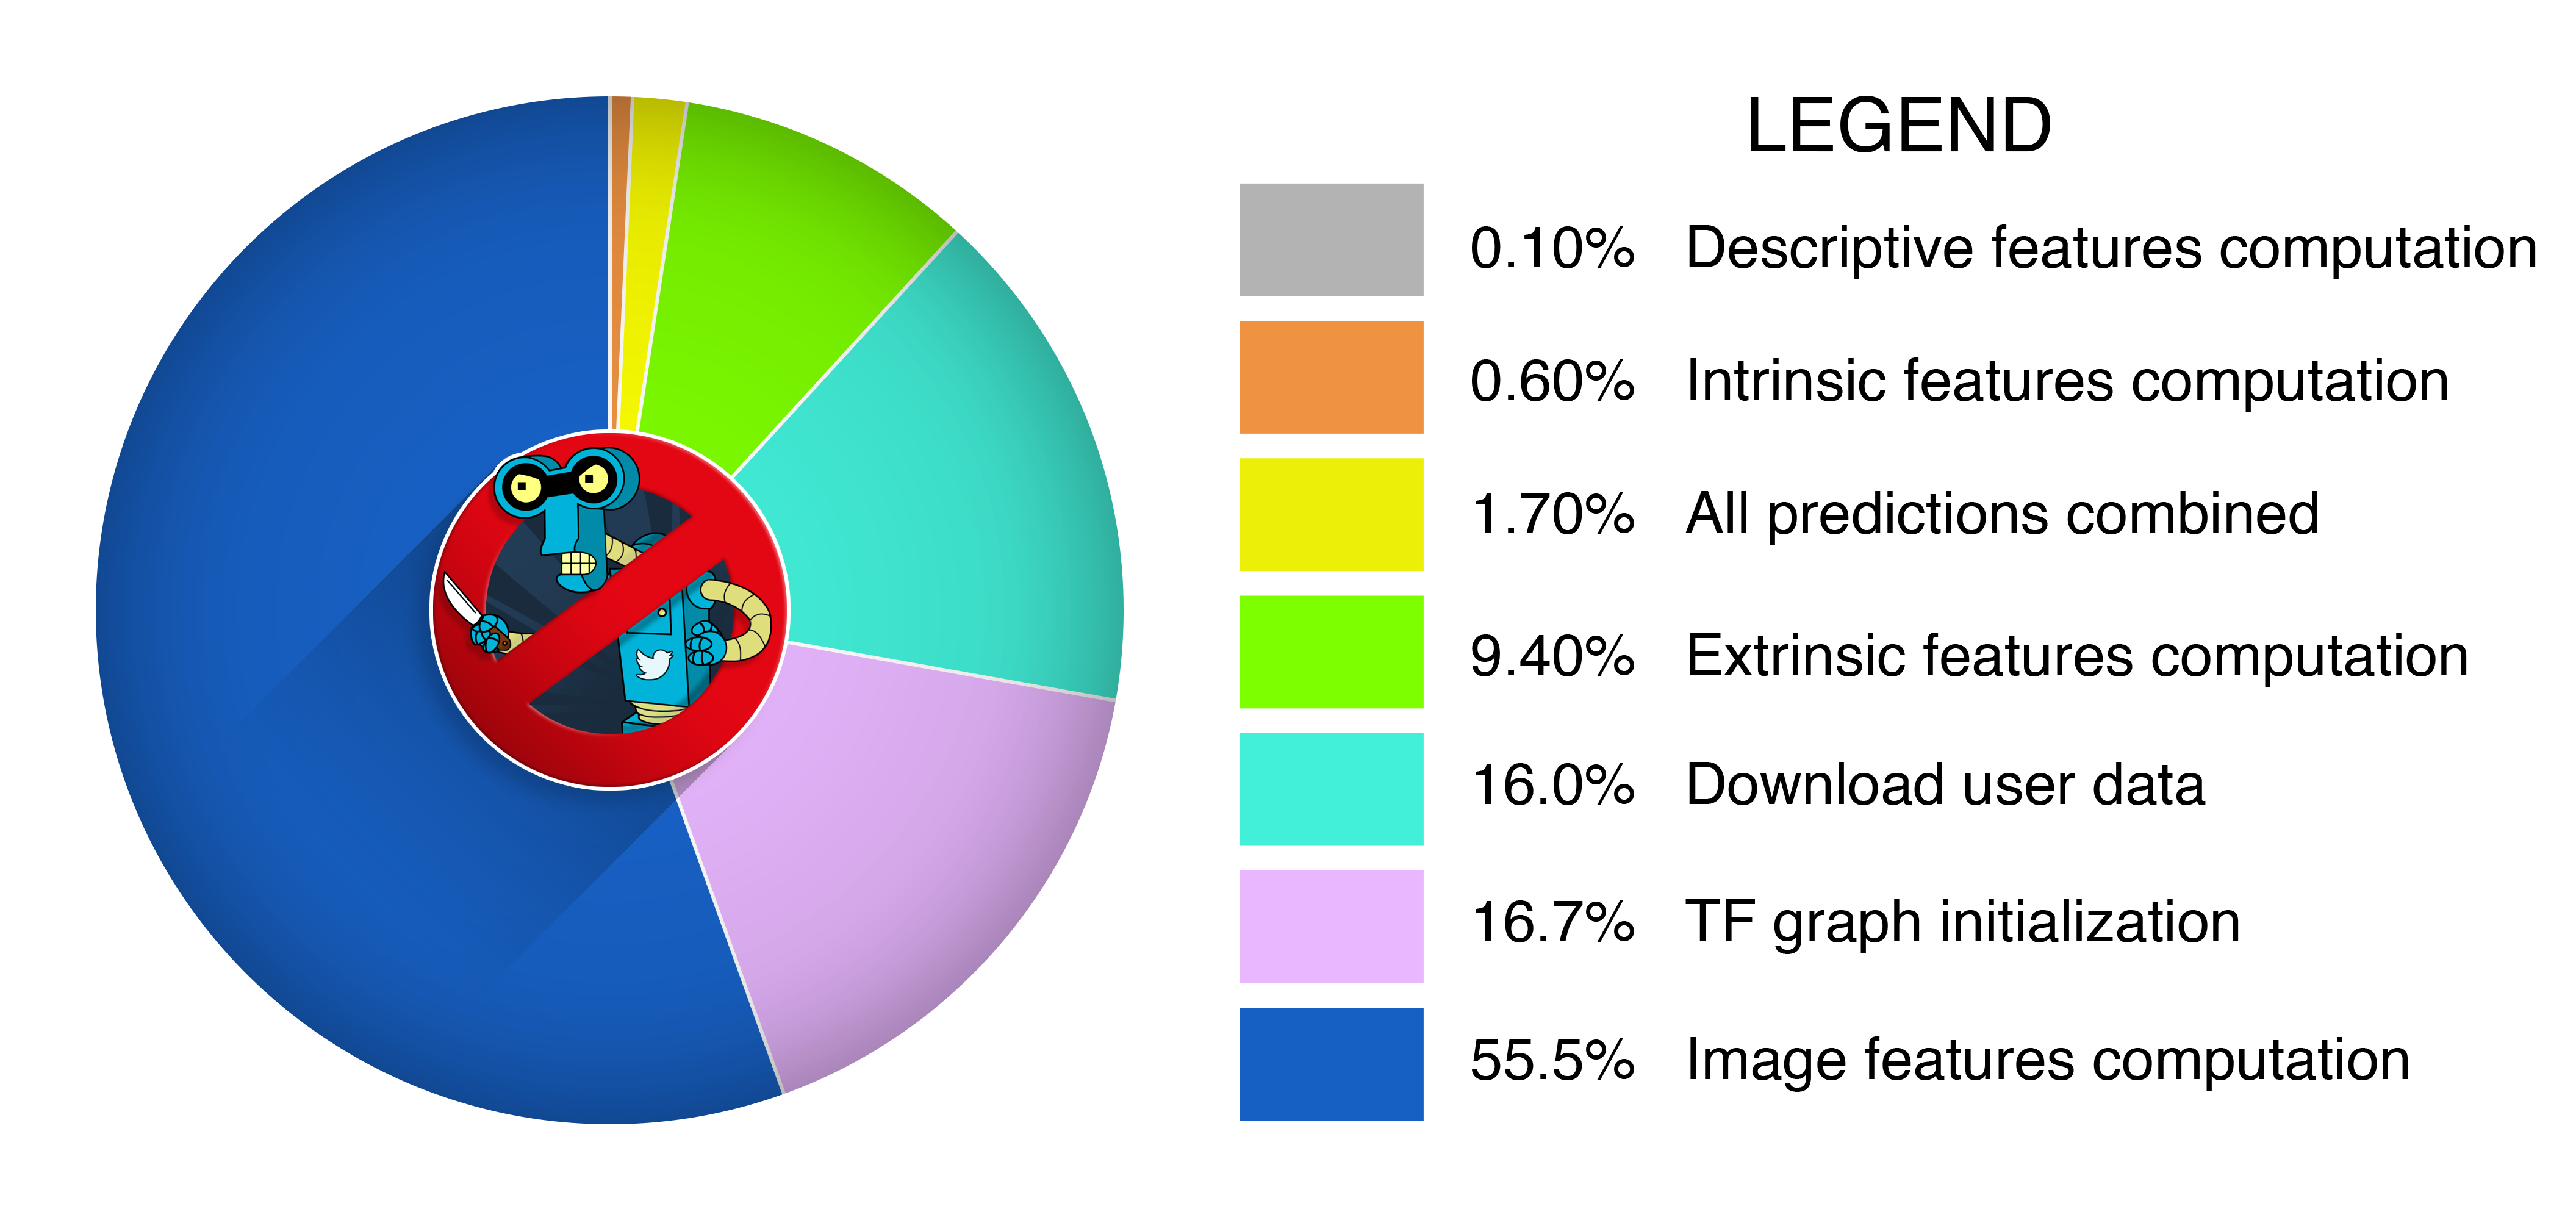
\includegraphics[width=\columnwidth]{chapter7/figure/time-pie.png}
	\end{center}
	\caption{Prediction time pie chart}
	\label{fig:pie}
\end{figure}

\subsection{Engine}
The real engine of the web application is a Python 3 script. It performs all the steps described in the pipeline execution section \ref{predicion_pipeline}.
The models, that have been previously fitted with data, serialized and stored, are now loaded by the Python script. They have to perform a single prediction at a time.
In addition to the models we built for the classification, the pre-trained convolutional neural network for NSFW recognition has been introduced to the pipeline, in order to infer on the media contents posted by the examined user.
The first step consists in calling the Twitter APIs to retrieve user's data and its most recent tweets, up to 100. 
The script, then, handles the preprocessing stages and the data preparations needed by the different classifiers.
Two final predictions are computed: the binary and the mutliclass classification.
The probability given to the bot target, by the binary classifier, is used to weight the mutliclass prediction provided by the stacking ensemble.
The final classification is composed by five probabilities: \textbf{P\textsubscript{NSWF},} \textbf{P\textsubscript{News-Spreader}}, \textbf{P\textsubscript{Spam-Bot}}, \textbf{P\textsubscript{Fake-Followers}}, \textbf{P\textsubscript{Genuine}}.
\subsection{Flask}
Flask is a web framework for Python. It is a good fit for our tool, due to the Python-based script of the engine.
The idea behind the Flask backend is to map URL paths to some logic we want to execute. In the flask main script, we used three endpoints to trigger the computation of some code.

\begin{itemize}
	\item[\PencilRight] \textit{@app.route}('\textbf{/}', methods=['GET']):\\
	This first endpoint is used to catch a HTTP GET request from the client browser.
	It gets triggered as the user navigates to \textit{www.botbuster.it}. The code that is being executed simply handles the rendering of the static files that compose the frontend, in order to make the website visible for the user, at that URL. The homepage appears as shown in Figure \ref{fig:homepage}
	\begin{figure}[htp!]
		\begin{center}
			
\includegraphics[width=\columnwidth]{chapter7/figure/homepage.png}\par 
		\end{center}
		\caption{BotBuster - homepage}
		\label{fig:homepage}
	\end{figure}
	\item[\PencilRight] \textit{@app.route}('\textbf{/api/user}', methods=['POST']):\\
	 Everytime a user fills the Twitter username input filed and click on "\textbf{Bust it}" button, a HTTP POST request is made and this endpoint is involved to execute the first part of the classification script, which retrieves the data regarding the requested Twitter account, with the official APIs. This first stage returns informations such as the profile picture, the nickname, the extended name, the number of tweets of that user, its following and follower accounts and its number of given likes, to someone else's contents.
	 All these data are wrapped into URL links, which bring the user to the Twitter pages dedicated to those data. together with the meta-data bar of the requested account, a GIF is displayed to inform the user that the classification is in pending status, as shown in Figure \ref{fig:user}.
	 \begin{figure}[htp!]
	 	\begin{center}
	 		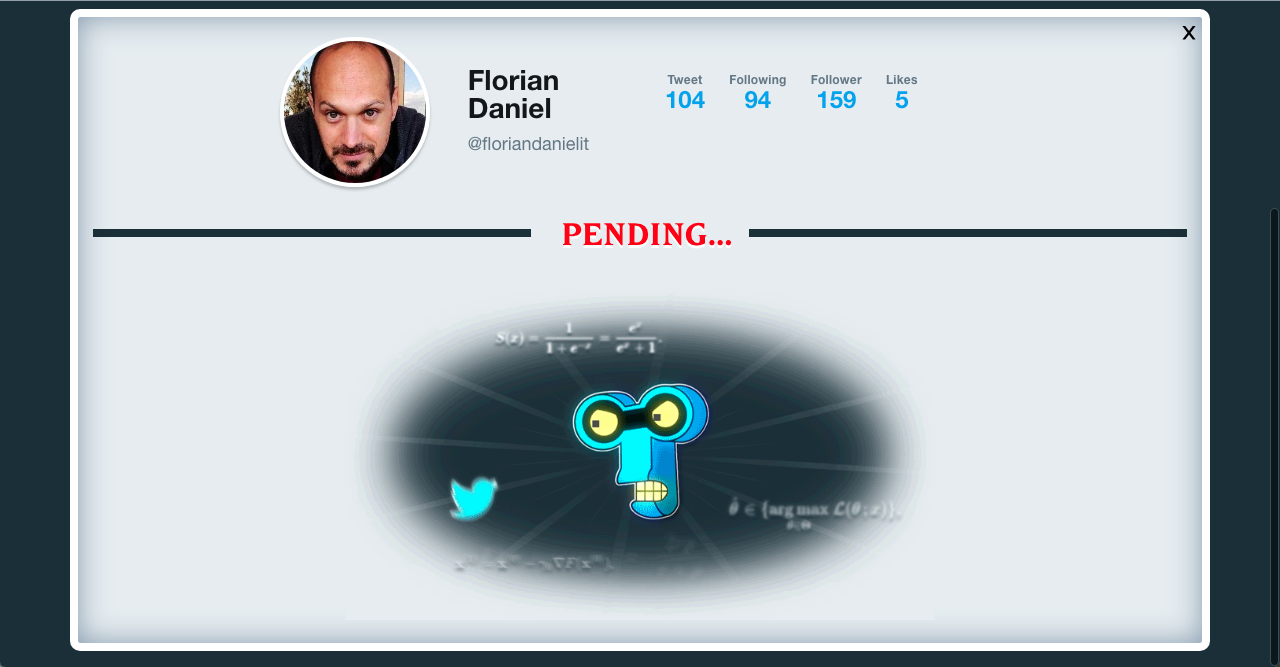
\includegraphics[width=\columnwidth]{chapter7/figure/user.png}\par 
	 	\end{center}
	 	\caption{BotBuster - pending classification}
	 	\label{fig:user}
	 \end{figure}
	\item[\PencilRight] \textit{@app.route}('\textbf{/api/classify}', methods=['POST']):\\
	This last endpoint is used subsequently to the previous one and it launches the classification script. It takes some seconds to compute the probabilities and to give them back to the client frontend. The prediction time may vary, as it depends on the number of media found in the account's tweets: the Inception convolutional neural network takes few seconds for each pictures it has to analyse. Once the computation is done, the resulting probabilities are returned as a JSON file to the client, in order to be rendered in the browser window, by the Angular frontend.
	The response provided by the classification script is represented as shown in Figure \ref{fig:classify}.
	 \begin{figure}[htp!]
		\begin{center}
			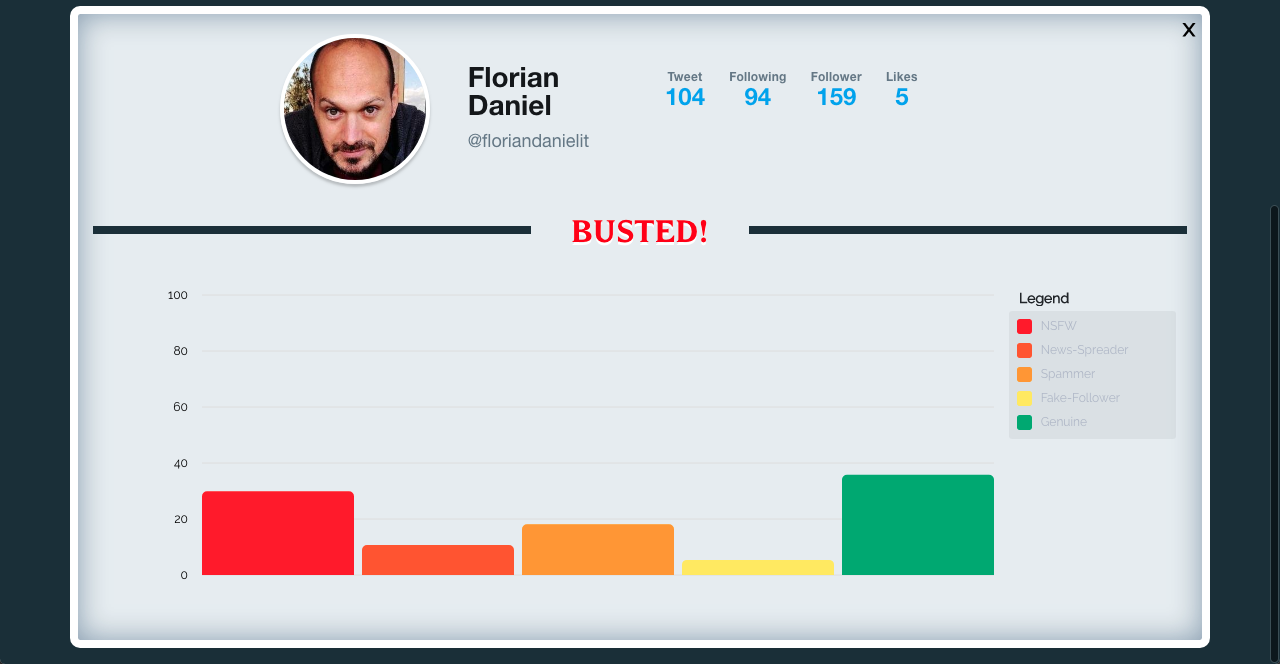
\includegraphics[width=\columnwidth]{chapter7/figure/classify.png}\par
		\end{center}
		\caption{BotBuster - classification}
		\label{fig:classify}
	\end{figure}
\end{itemize}

\section{Frontend}
The client-side application relies on Angular framework, a TypeScript-based open source, frontend web application platform, developed for the most by Google and some individuals and developer corporations.
It is a rebuild of the previous AngularJS framework.
BotBuster fronted project is composed by a single HTML page, with TypeScript files creating complex types for the data and handling the HTTP responses.
The angular component operating on the homepage contains HTML tags that are being toggled with the responses provided by the web server application.

As soon as the user submits a Twitter username trough the input field, the search bar gets hidden and the meta-data of the requested account appears, together with the pending GIF. Once the last POST (the classification request) gets a response, the pending GIF disappears to be replaced with the charts representing the classes and their assigned probabilities. 
Angular framework makes TypeScript files work with the web browser, thanks to Javascript language, and it loads the components without loading the entire pages to do it. It fits our purpose, since we didn't need many pages to be displayed and we wanted a light visualization of the script results.

\section{Deployment platform}
The platform used for the deployment is the App Engine of the Google Cloud Platform.
The application is being deployed, along with the needed packages and dependencies, on a Python flexible environment.
Then, the domain \textbf{www.botbuster.it} has been redirected to point to the address of the web application provided by Google, in order to have a user friendly URL visible on the web.
\section{Comparison with Botometer}
Our work differs from the Botometer project due the effort involved in deepening the classifications among bots and the detection of their harmful behaviours.
However, since the first element of our prediction pipeline is built also with the same data used for Botometer, we wanted some comparison terms on real world cases.

We analysed some specific accounts, in order to highlights the main difference between our predictions and theirs, as well as the similarities.
The comparison in Figure \ref{fig:cnn} shows the differences between our methods and theirs, with a verified account, such as an official editorial user.
In this case, we examined the CNN account. Although this account is marked as verified by Twitter itself, it is reasonable to believe it is managed by automations. These kinds of profiles are directly linked with the official editors' websites and they tweet the same contents found in their online newspapers. Such linked behaviour could be easily programmed, in order to guarantee a high rate of tweeting activity.
The verified mark has been used as a feature even in our binary model, but we lacked lots of values for that attributes, so, in our classification, it doesn't play an important role in assessing the authenticity to the profiles.
\begin{figure}[htp!]
	\begin{center}
		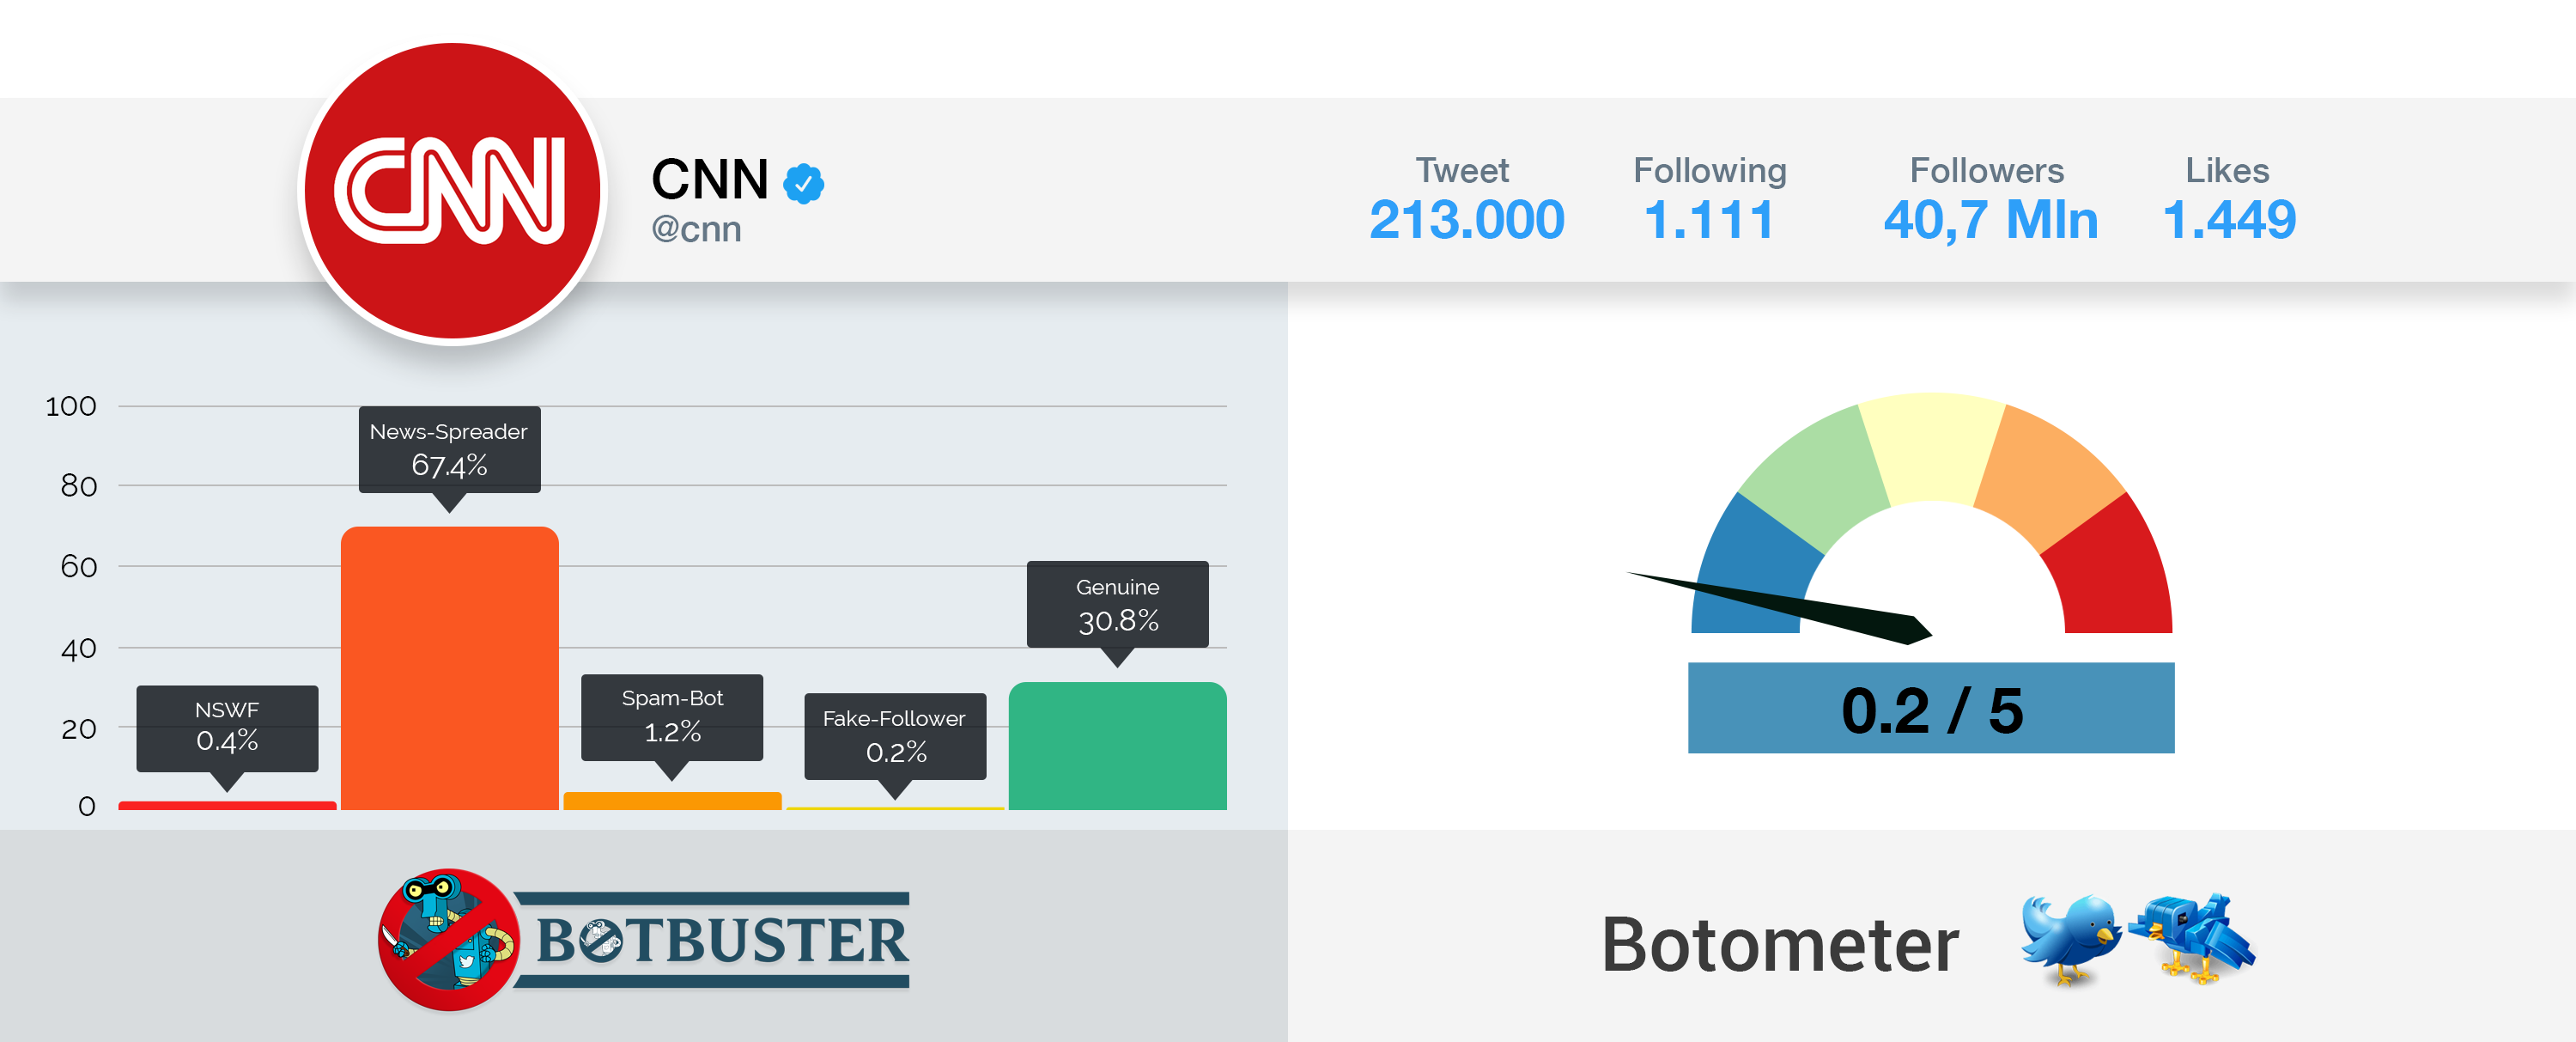
\includegraphics[width=\columnwidth]{chapter7/figure/cnn.png}\par
	\end{center}
	\caption{BotBuster vs Botometer - CNN's account comparison}
	\label{fig:cnn}
\end{figure}
We think that Botometer relies heavily on the verified feature to detect genuine accounts, since lots of the verified account tested with that tool have been evaluated as legitimate. Figure \ref{fig:verified} shows this particular behaviour of the Botometer web application. All the account shown are likely automated or act in a way that is not recognizable as a human interaction on the social platform. Their tweeting frequency should discourage the classifier to blindly trust the verified attribute.
\begin{figure}[htp!]
	\begin{center}
		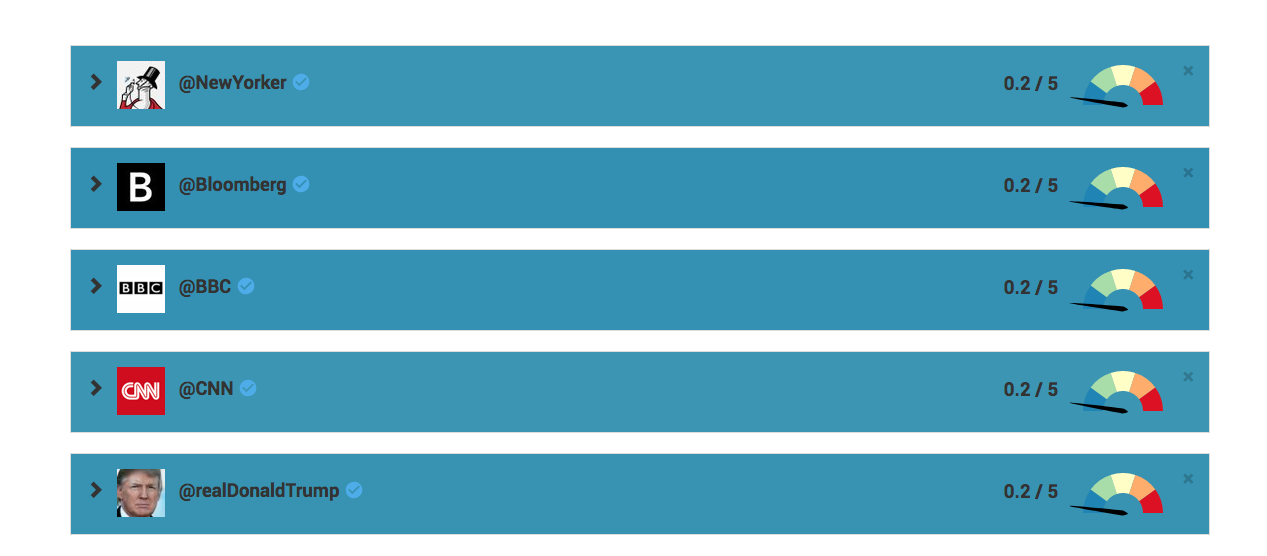
\includegraphics[width=\columnwidth]{chapter7/figure/verified.png}\par
	\end{center}
	\caption{Verified accounts classification with Botometer}
	\label{fig:verified}
\end{figure}
We couldn't be sure that verified accounts are handled by bots neither, but we chose to let the Random Forest weight that feature basing it on the information gain, as it does with all the other attributes.
The inner mutliclass classification matches our expectations, since this account's goal is to spread its news, and we identified it as a News-Spreader, with 67.4\% of confidence.
As we get deeper in our prediction, we can observe the feature values computed for that examined profile. In particular, the intrinsic and the extrinsic features seem to frame the profile nature well:
\begin{center}
	\begin{tabular}{@{}c|c|c|c@{}}
		\multicolumn{4}{c}{Extrinsic features} \\
		\hline
		\multicolumn{1}{c|}{\textbf{NSFW score}} & 
		\multicolumn{1}{c|}{\textbf{NS score}} & 
		\multicolumn{1}{c|}{\textbf{SB score}} & 
		\multicolumn{1}{c}{\textbf{FF score}}\\
		\hline
		\multicolumn{1}{c|}{0.002} &
		\multicolumn{1}{c|}{0.034} &
		\multicolumn{1}{c|}{0.011} &
		\multicolumn{1}{c}{0.011} \\
		\hline
	\end{tabular}
\end{center}
\begin{center}
	\begin{tabular}{@{}c|c@{}}
		\multicolumn{2}{c}{Intrinsic features} \\
		\hline
		\multicolumn{1}{c|}{\textbf{Tweet intradistance}} & 
		\multicolumn{1}{c}{\textbf{URL entropy}}\\
		\hline
		\multicolumn{1}{c|}{18.25} &
		\multicolumn{1}{c}{0.0}\\
		\hline
	\end{tabular}
\end{center}

The News\_spreader\_words\_score is the highest among the multiclass extrinsic features, this means that the words used by the CNN accounts matches, for the most, the ones collected in our News-Spreaders dictionary. Moreover, we can see that the URL entropy is equal to zero, and this means two possibilities: the account has no tweets with links on its timeline or it tweets the same URL in each post. The last option is the one standing for this case. The last 100 tweets retrieved contain the link to the CNN official website.

Another difference between our work and Botometer is represented in Figure \ref{fig:fake}, where a user that we detect as a Fake-Follower can't be classified by Botometer, because of the absence of tweets on its timeline. This could mean that the researcher behind that project thought that the user features weren't enough to perform a proper prediction, without data coming by the tweeting activity.
We chose to not use the tweeting mechanism as a support feature, being aware that user driven classification could be less precise, due to the limited information obtained by the user profile only.
\begin{figure}[htp!]
	\begin{center}
		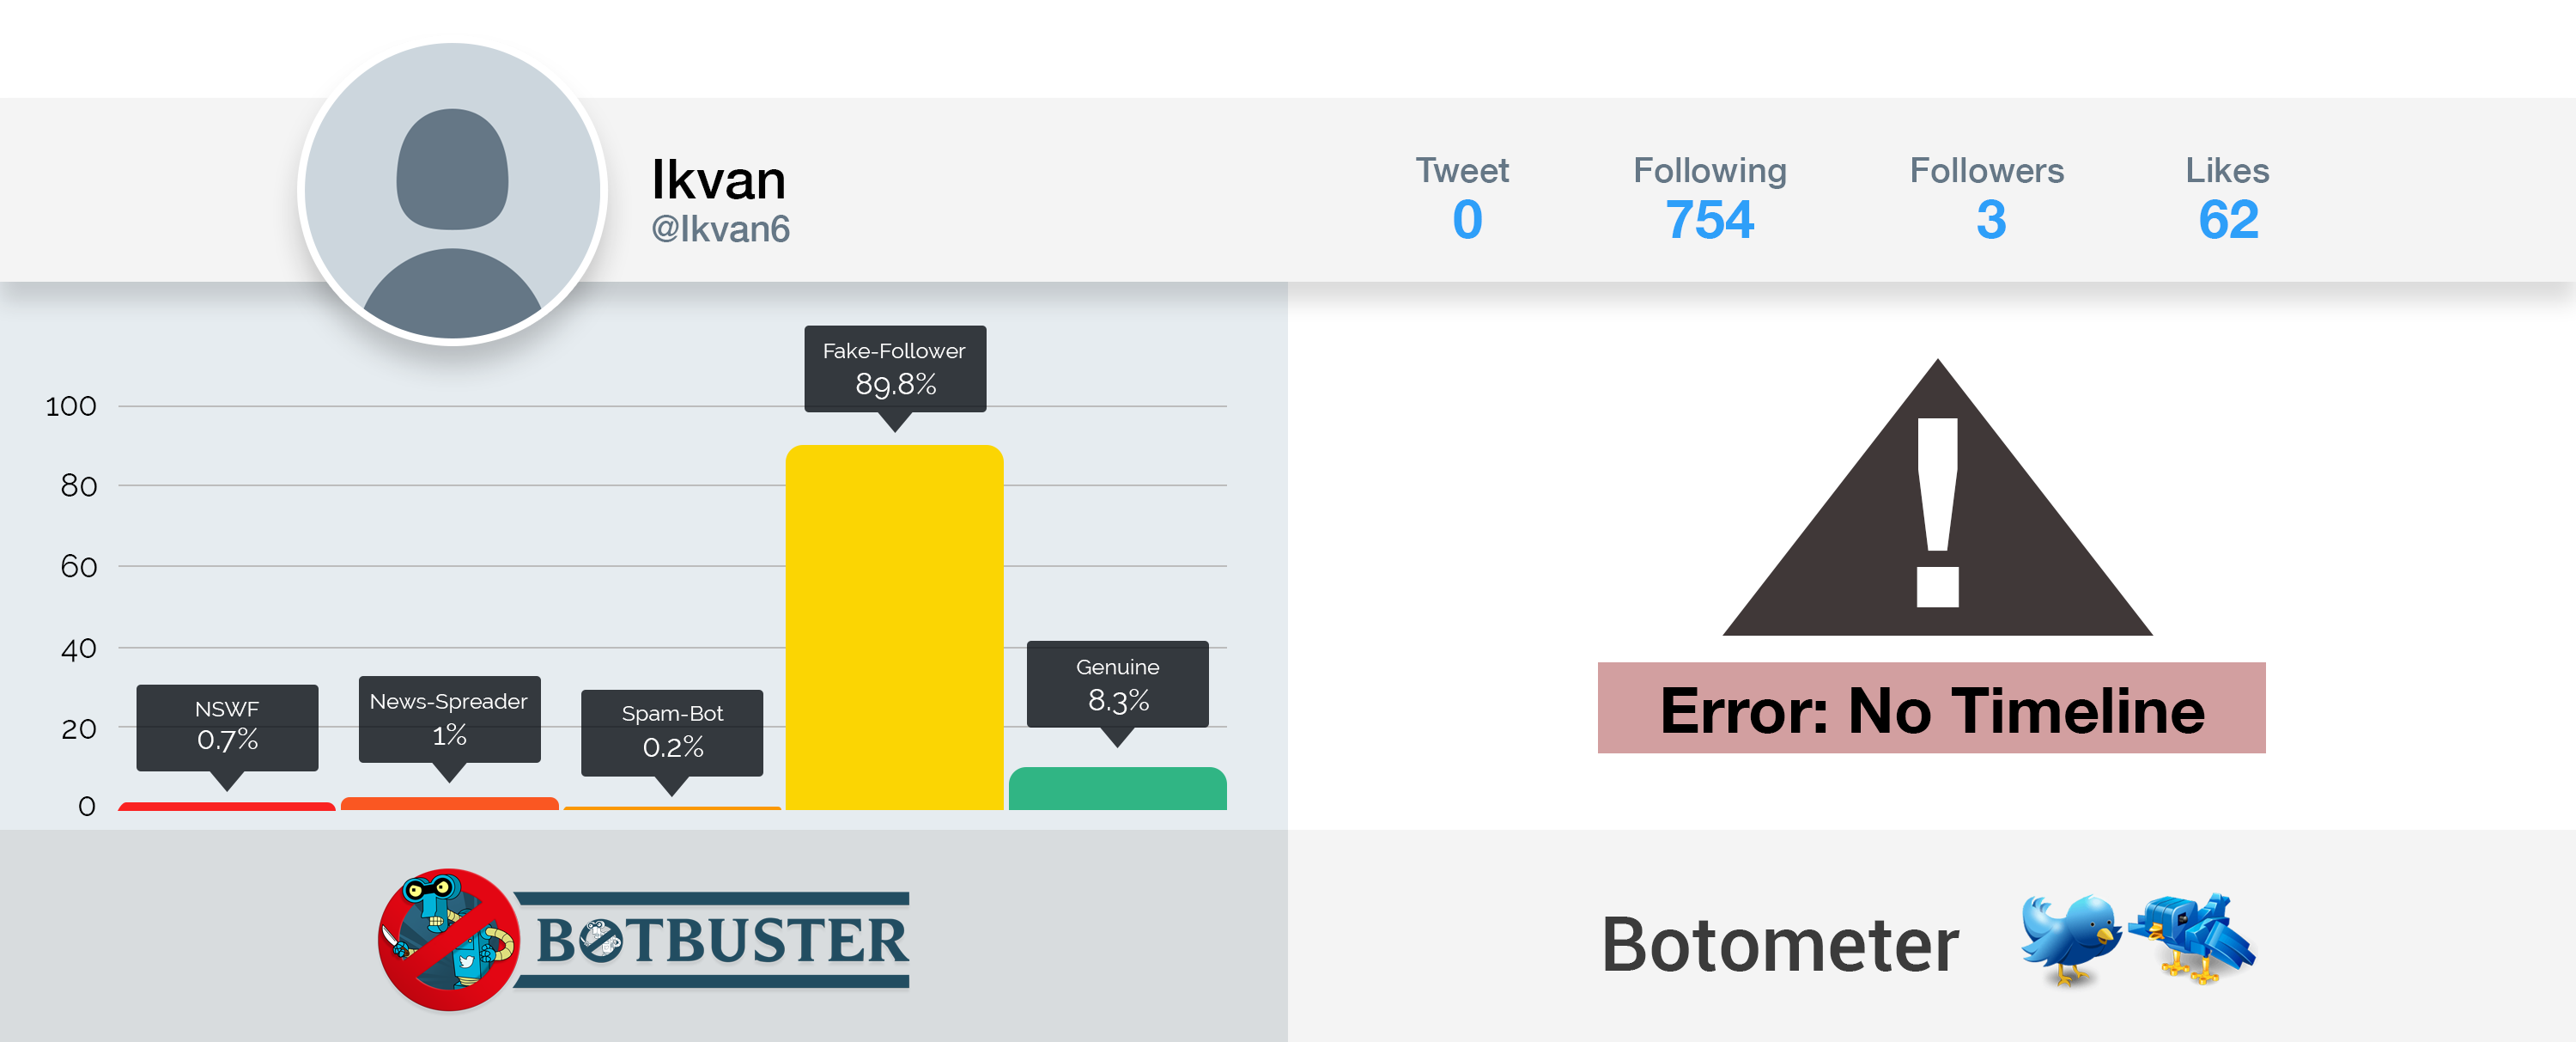
\includegraphics[width=\columnwidth]{chapter7/figure/fake_follower.png}\par
	\end{center}
	\caption{Classification of users without tweets on their timelines}
	\label{fig:fake}
\end{figure}

\begin{figure}[htp!]
	\begin{center}
		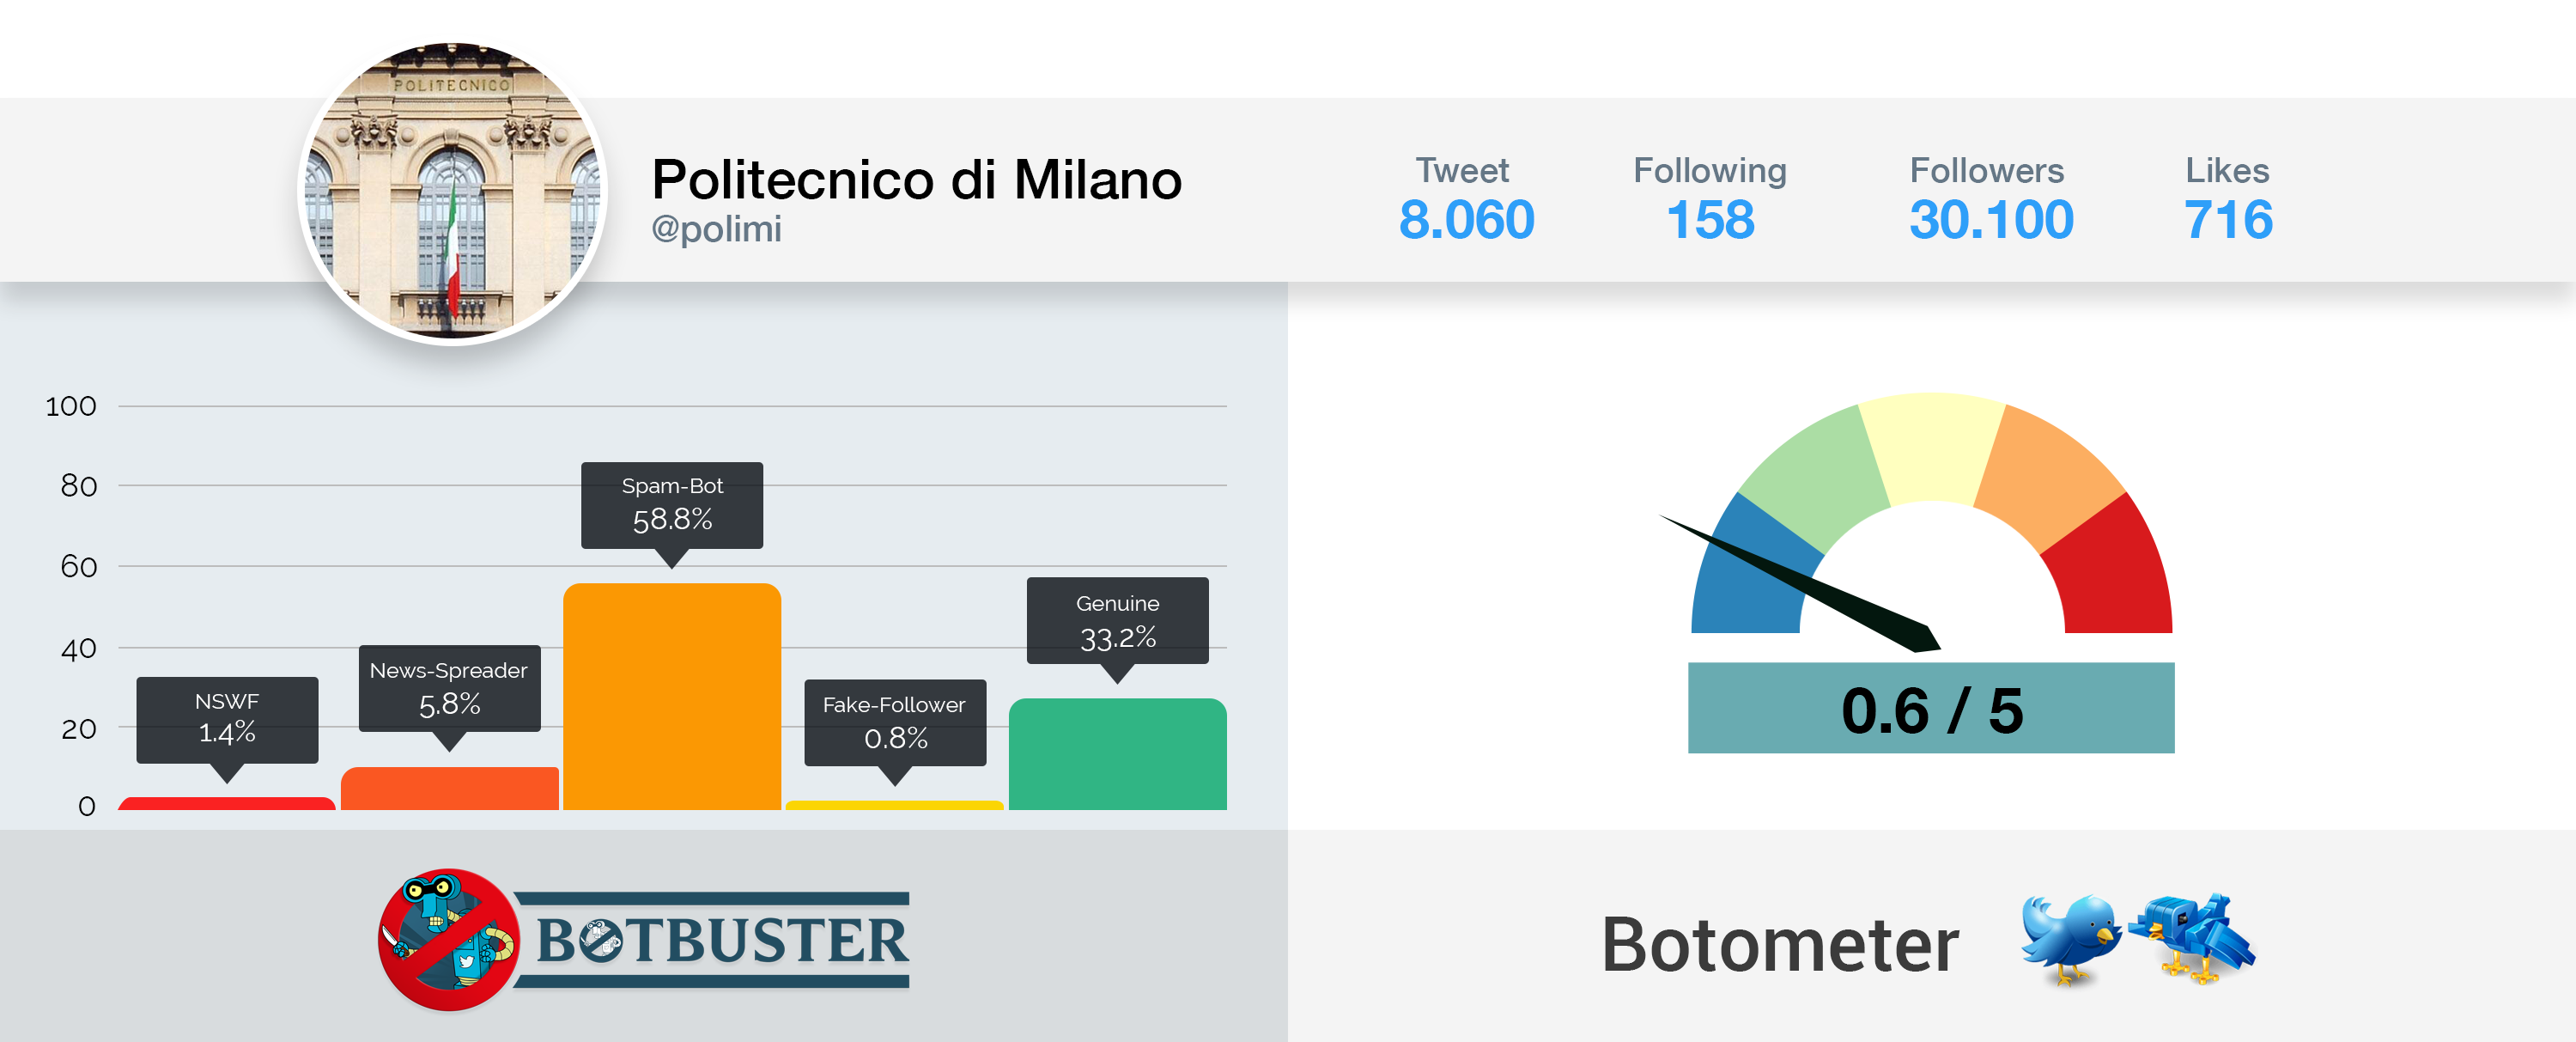
\includegraphics[width=\columnwidth]{chapter7/figure/polimi.png}\par
	\end{center}
	\caption{Comparison of PoliMi account classifications}
	\label{fig:polimi}
\end{figure}

In Figure \ref{fig:polimi}, instead, Botometer seems to perform better with this type of accounts. We examined the official profile of PoliMi. Botometer detects it as legitimate, but we sees it as a Spam-Bot, principally, with a good percentage of genuine nature. This difference cannot be imputed to the verified check, as it is missing, in this example.
Looking at the partial scores assigned by the feature groups that Botometer computes, we can see that it assigns very low bot-likely values in the Sentiment field, as well as in the Network lookup. Figure \ref{fig:polimi_details} shows the partial scores assigned to PoliMi account. They implemented \textit{English-specific features} and \textit{Language-independent features} too; we didn't perform this distinction, every textual feature, as well as the words used for the text-based classifier, can be seen as their Language-independent attributes. The issue with this approach is the majority language collected in our training data. Most of the accounts gathered are English speakers, this leads to English-oriented dictionaries and textual features, making the classification of foreign accounts harder for our tool.
\begin{figure}[htp!]
	\begin{center}
		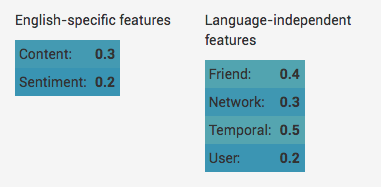
\includegraphics[width=0.8\columnwidth]{chapter7/figure/polimi_details.png}\par
	\end{center}
	\caption{Partial Botometer scores for PoliMi account}
	\label{fig:polimi_details}
\end{figure}

Since it is legitimate to think that this profile is managed by a real person, we consider those feature introduced by Botometer as a valid contribute to the binary classifier. It could be considered in future implementations, in order to better distinguish human profiles, even with very high tweeting activities.

During the tool testing, we noticed some particular types of users that we didn't be able to include in the training sets. These types are the \textit{protected} users and the ones which never had interactions on the social, at all. No interactions means that these unused users have no tweets, no followings, no followers, no likes and often no profile picture.
Protected users choose to hide their sharing activities to everyone, and to reveal their timelines only to those accounts who send them the request to see their tweets. Obviously, the timelines aren't accessible via Twitter APIs, so it is hard to infer the nature of such accounts, since it is not possible to asses if they post contents or not. For this kind of users, we decided to assign a standard classification, that represents the uncertainty, as shown in Figure \ref{fig:protected}. The classification assesses a 50\% probabilities to both bot and genuine categories, and partitions the bot behaviours in equal parts.
Instead, the prediction output of unused accounts has been fixed with a 100\% chance to be genuine. We cannot assess the real nature of those users, nor their purpose, but we can state that their not harmful, since they do not have interactions with other accounts. That makes them genuine accounts, like legitimate users, they don't represent threats or harmful entities. An example of such classification is shown in Figure \ref{fig:empty}.

\begin{figure}[htp!]
	\centering 
	\subfigure[Protected account]{
		\label{fig:protected}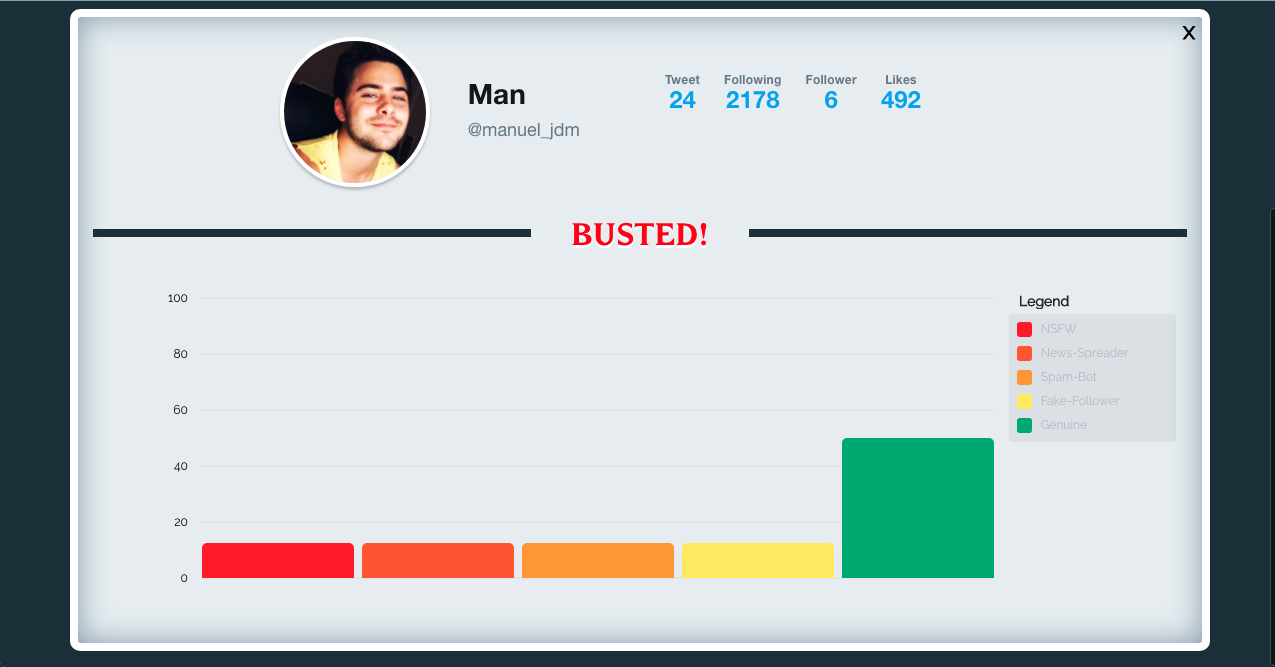
\includegraphics[width=60mm]{chapter7/figure/protected.png}}
	\subfigure[Unused account]{
		\label{fig:empty}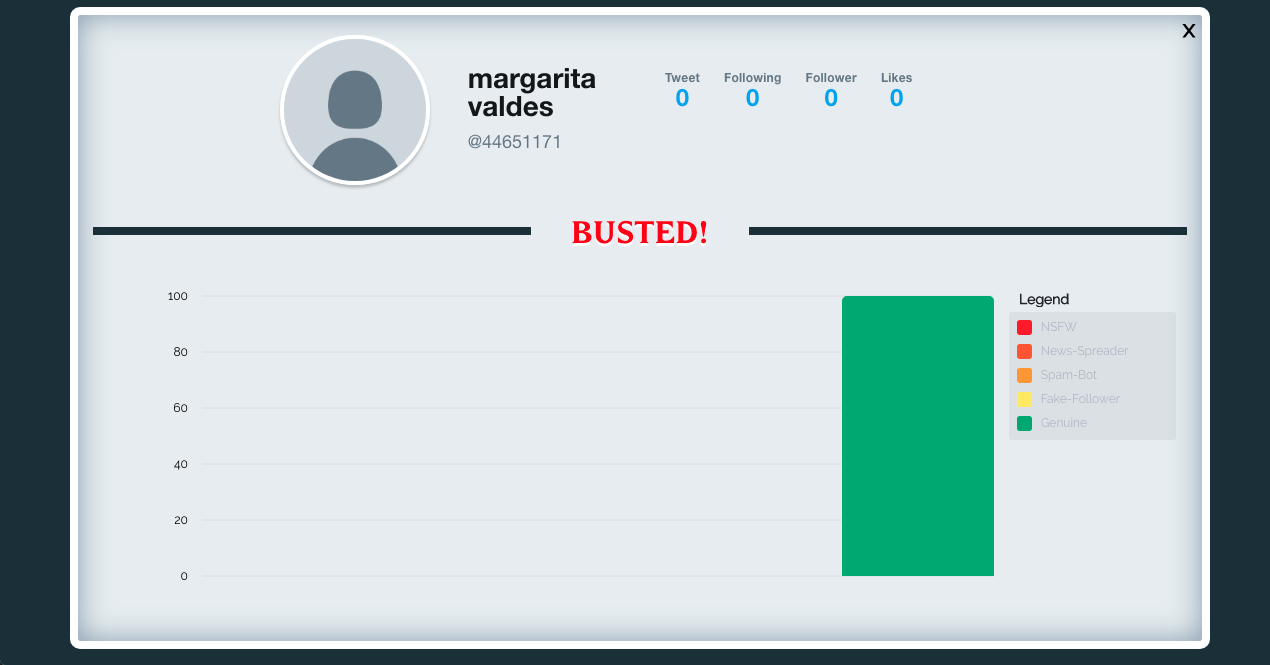
\includegraphics[width=60mm]{chapter7/figure/empty.png}}
	\caption{Classification of specific account types}
\end{figure}
